\documentclass[border=10pt]{standalone}
\usepackage{pgfplots}
\pgfplotsset{compat=1.18}
\begin{document}
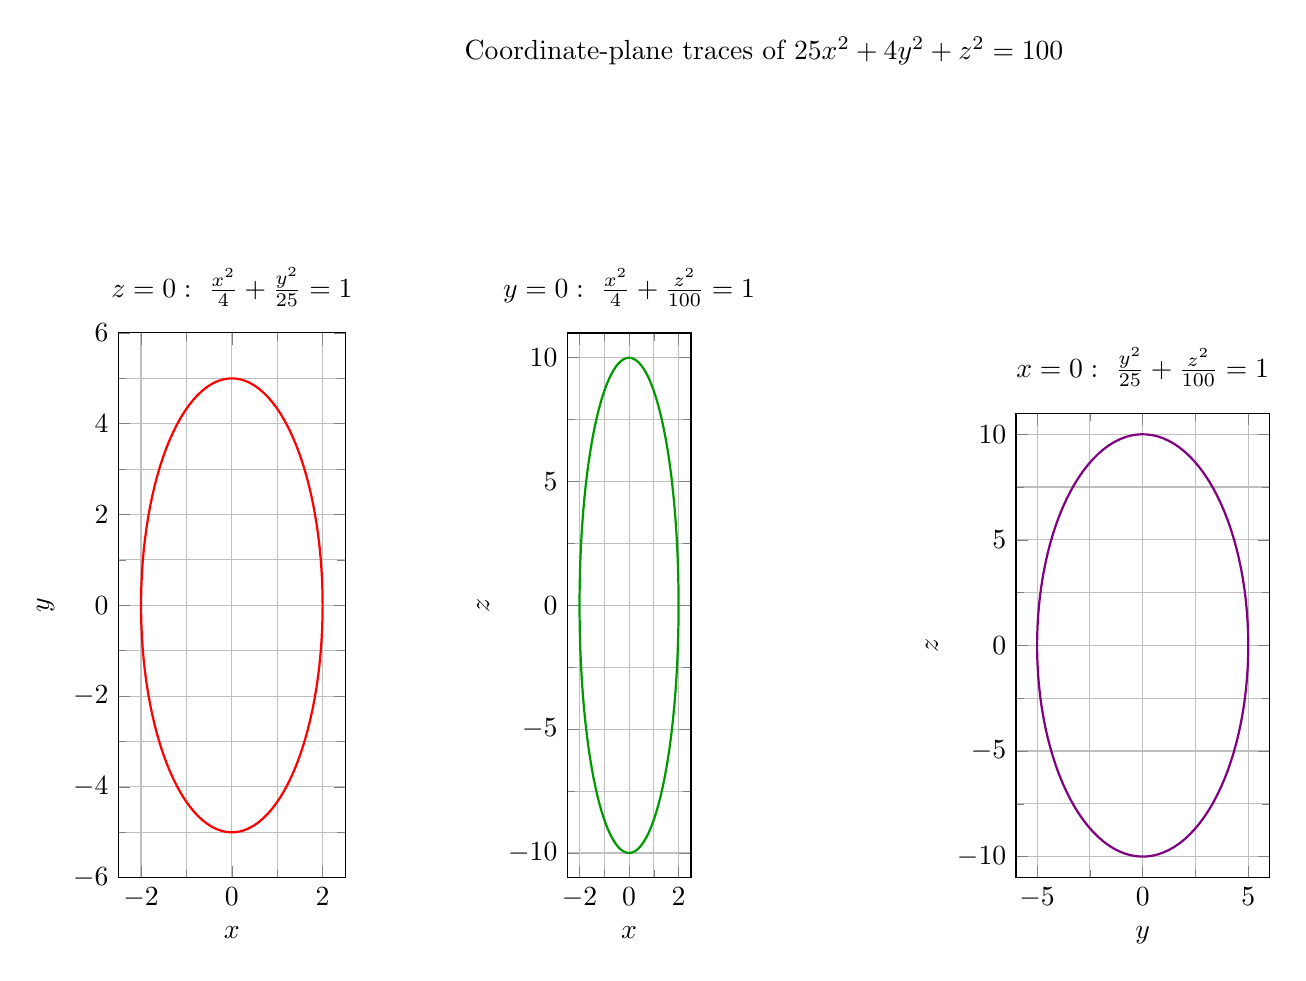
\begin{tikzpicture}
\node[anchor=south] at (8.2cm,10.2cm) {Coordinate-plane traces of $25x^2+4y^2+z^2=100$};

\begin{axis}[
  at={(0,0)},
  anchor=south west,
  width=4.8cm, height=8.5cm,
  xlabel={$x$}, ylabel={$y$},
  xmin=-2.5, xmax=2.5, ymin=-6, ymax=6,
  grid=both,
  minor tick num=1,
  title={$z=0:\ \frac{x^2}{4}+\frac{y^2}{25}=1$},
  axis equal image=true,
]
\addplot[domain=0:360, samples=120, red, thick] ({2*cos(x)}, {5*sin(x)});
\end{axis}

\begin{axis}[
  at={(5.7cm,0)},
  anchor=south west,
  width=4.8cm, height=8.5cm,
  xlabel={$x$}, ylabel={$z$},
  xmin=-2.5, xmax=2.5, ymin=-11, ymax=11,
  grid=both,
  minor tick num=1,
  title={$y=0:\ \frac{x^2}{4}+\frac{z^2}{100}=1$},
  axis equal image=true,
]
\addplot[domain=0:360, samples=120, green!60!black, thick] ({2*cos(x)}, {10*sin(x)});
\end{axis}

\begin{axis}[
  at={(11.4cm,0)},
  anchor=south west,
  width=4.8cm, height=8.5cm,
  xlabel={$y$}, ylabel={$z$},
  xmin=-6, xmax=6, ymin=-11, ymax=11,
  grid=both,
  minor tick num=1,
  title={$x=0:\ \frac{y^2}{25}+\frac{z^2}{100}=1$},
  axis equal image=true,
]
\addplot[domain=0:360, samples=120, violet, thick] ({5*cos(x)}, {10*sin(x)});
\end{axis}
\end{tikzpicture}
\end{document}